\documentclass[twoside,10pt]{article}
\usepackage{amsmath,amsfonts,amsthm,fullpage}
\usepackage{mymath}
\usepackage{algorithm}
\usepackage{algorithmic}
\usepackage{graphicx}


\begin{document}

\title{CS 7641 CSE/ISYE 6740 Homework 1}
\author{Le Song}
\date{Deadline: Sep. 22 Tue, 11:55pm}
\maketitle

\begin{itemize}
  \item Submit your answers as an electronic copy on T-square.
  \item No unapproved extension of deadline is allowed. Zero credit will be assigned for late submissions. Email request for late submission may not be replied.
  \item For typed answers with LaTeX (recommended) or word processors, extra credits will be given. If you handwrite, try to be clear as much as possible. No credit may be given to unreadable handwriting.
  \item Explicitly mention your collaborators if any.
  \item Recommended reading: PRML\footnote{Christopher M. Bishop, Pattern Recognition and Machine
Learning, 2006, Springer.} Section 9.1, 12.1
\end{itemize}

%----------------------------------------------------------------------------------
\section{Probability [15 pts]}

\subsubsection*{(a) Stores A, B, and C have 50, 75, and 100 employees and, respectively, 50, 60, and 70 percent of these are women. Resignations are equally likely among all employees, regardless of stores and sex. Suppose an employee resigned, and this was a woman. What is the probability that she has worked in store C? [5 pts]}

\subsubsection*{(b) A laboratory blood test is 95 percent effective in detecting a certain disease when it is, in fact, present. The test also yields a false positive result for 1 percent of the healthy persons tested. That is, if a healthy person is tested then with probability 0.01 the test result will imply he has the disease. If 0.5 percent of the population actually has the disease, what is the probability a person has the disease given that his test result is positive? [5 pts]}

\textbf{[c-d]} On the morning of September 31, 1982, the won-lost records of the three leading baseball teams in the western division of the National League of the United States were as follows:

\begin{table}[!h]
\centering \small
\begin{tabular}{l|c|c}
  \hline
  Team & Won & Lost\\
  \hline \hline
  Atlanta Braves & 87 & 72\\
  San Francisco Giants & 86 & 73\\
  Los Angeles Dodgers & 86 & 73\\
  \hline
\end{tabular}
\end{table}

Each team had 3 games remaining to be played. All 3 of the Giants games were with the Dodgers, and the 3 remaining games of the Braves were against the San Diego Padres. Suppose that the outcomes of all remaining games are independent and each game is equally likely to be won by either participant. If two teams tie for first place, they have a playoff game, which each team has an equal chance of winning.

\subsubsection*{(c) What is the probability that Atlanta Braves wins the division? [2 pts]}
\subsubsection*{(d) What is the probability to have an additional playoff game? [3 pts]}
%\vspace{1cm}
\newpage

%----------------------------------------------------------------------------------
\section{Maximum Likelihood [15 pts]}

Suppose we have $n$ i.i.d (independent and identically distributed)
data samples from the following probability distribution. This
problem asks you to build a log-likelihood function, and find the
maximum likelihood estimator of the parameter(s).

\subsubsection*{(a) Poisson distribution [5 pts]}
The Poisson distribution is defined as
\begin{equation} \nonumber
P(x_i = k) = \frac{\lambda^k e^{-\lambda}}{k!} (k = 0, 1, 2, ...).
\end{equation}
What is the maximum likelihood estimator of $\lambda$?

\subsubsection*{(b) Multinomial distribution [5 pts]}
The probability density function of Multinomial distribution is given by 
$$f(x_1,x_2,\dots,x_k;n,\theta_1,\theta_2,\dots,\theta_k)=\frac{n!}{x_1!x_2!\cdots x_k!}\prod_{j=1}^{k}\theta_j^{x_j},$$
where $\sum_{j=1}^k\theta_j=1,\sum_{j=1}^k x_j=n$. What is the maximum likelihood estimator of $\theta_j, j=1,\dots k$?

\subsubsection*{(c) Gaussian normal distribution [5 pts]}
Suppose we have $n$ i.i.d (Independent and Identically Distributed)
data samples from a univariate Gaussian normal distribution
$\mathcal{N}(\mu, \sigma^2)$, which is given by
\begin{equation}
\mathcal{N}(x; \mu, \sigma^2) = \frac{1}{\sigma \sqrt{2\pi}} \exp
\left( - \frac{(x - \mu)^2}{2\sigma^2} \right).\nonumber
\end{equation}
What is the maximum likelihood estimator of $\mu$ and $\sigma^2$?
\vspace{1cm}

\iffalse
\subsubsection*{(b) Exponential distribution [5 pts]}
The probability density function of Exponential distribution is
given by
\begin{equation} \nonumber
f(x) = \left\{\begin{matrix}
\lambda e^{-\lambda x} & x \ge 0\\
0 & x < 0
\end{matrix}\right.
\end{equation}
What is the maximum likelihood estimator of $\lambda$?
\fi

%----------------------------------------------------------------------------------
\section{Principal Component Analysis [20 pts]}
In class, we learned that Principal Component Analysis (PCA)
preserves variance as much as possible. We are going to explore
another way of deriving it: minimizing reconstruction error.

Consider data points $\text x^n (n=1, ..., N)$ in $D$-dimensional space.
We are going to represent them in $\{\text u_1, ..., \text u_D\}$ orthonormal basis.
That is,
\begin{equation} \nonumber
\text x^n = \sum_{i=1}^D \alpha_i^n \text u_i = \sum_{i=1}^D ({\text x^n}^T \text u_i) \text u_i.
\end{equation}
Here, $\alpha^n_i$ is the length when $\text x^n$ is projected onto
$u_i$.

Suppose we want to reduce the dimension from $D$ to $M < D$. Then
the data point $\text x^n$ is approximated by
\begin{equation} \nonumber
\tilde{\text x}^n = \sum_{i=1}^M z_i^n \text u_i + \sum_{i=M+1}^D b_i \text u_i.
\end{equation}
In this representation, the first $M$ directions of $\text u_i$ are
allowed to have different coefficient $z^n_i$ for each data point,
while the rest has a constant coefficient $b_i$. As long as it is
the same value for all data points, it does not need to be 0.

Our goal is setting $\text u_i$, $z^n_i$, and $b_i$ for $n = 1,..., N$
and $i = 1, ..., D$ so as to minimize reconstruction error. That is,
we want to minimize the difference between $\text x^n$ and $\tilde{\text x}^n$ over $\{ \text u_i, z^n_i, b_i \}$:
\begin{equation} \nonumber
J = \frac{1}{N} \sum_{n=1}^N \| \text x^n - \tilde{\text x}^n \|^2.
\end{equation}

\subsubsection*{(a) What is the assignment of $z_j^n$ for $j=1, ..., M$ minimizing $J$? [5 pts]}
\subsubsection*{(b) What is the assignment of $b_j$ for $j=M+1, ..., D$ minimizing $J$? [5 pts]}
\subsubsection*{(c) Express optimal $\tilde{\text x}^n$ and $\text x^n - \tilde{\text x}^n$ using your answer for (a) and (b). [2 pts]}
\subsubsection*{(d) What should be the $\text u_i$ for $i=1, ..., D$ to minimize $J$? [8 pts]}

\emph{Hint:} Use $S = \frac{1}{N} \sum_{n=1}^N (\text x^n - \bar{\text x})(\text x^n -
\bar{\text x})^T$ for sample covariance matrix. \vspace{1cm}


%----------------------------------------------------------------------------------
\section{Clustering [20 pts]}

\textbf{[a-b]} Given $N$ data points $\text x^n (n=1,\dots,N)$, $K$-means clustering algorithm groups them into $K$ clusters by minimizing the distortion function over $\{ r^{nk}, \mu^k \}$
$$J=\sum_{n=1}^N\sum_{k=1}^Kr^{nk} \|\text x^n-\mu^k\|^2,$$
where $r^{nk}=1$ if $\text x^n$ belongs to the $k$-th cluster and $r^{nk}=0$ otherwise.

\subsubsection*{(a) Prove that using the squared Euclidean distance $\|\text x^n-\mu^k\|^2$ as the dissimilarity function and minimizing the distortion function, we will have 
   $$\mu^k=\frac{\sum_n r^{nk} \text x_n}{\sum_n r^{nk}}.$$
   That is, $\mu^k$ is the center of $k$-th cluster. [5 pts]}

\subsubsection*{(b) Prove that $K$-means algorithm converges to a local optimum in finite steps. [5 pts]}


\textbf{[c-d]} In class, we discussed bottom-up hierarchical clustering. For each iteration, we need to find two clusters $\{\text x_1, \text x_2, \dots, \text x_m\}$ and $\{\text y_1, \text y_2, \dots, \text y_p\}$ with the minimum distance to merge. Some of the most commonly used distance metrics between two clusters are:
    \begin{itemize}
    \item Single linkage: the minimum distance between any pairs of points from the two clusters, i.e.
    $$\min_{i=1,\dots,m \atop j=1,\dots, p}\|\text x_i - \text y_j\|$$
    \item Complete linkage: the maximum distance between any parts of points from the two clusters, i.e.
    $$\max_{i=1,\dots,m \atop j=1,\dots, p}\|\text x_i - \text y_j\|$$
    \item Average linkage: the average distance between all pair of points from the two clusters, i.e.
    $$\frac{1}{mp}\sum_{i=1}^m\sum_{j=1}^p\|\text x_i - \text y_j\|$$
    \end{itemize}

\subsubsection*{(c) When we use the bottom up hierarchical clustering to realize the partition of data, which of the three cluster distance metrics described above would most likely result in clusters most similar to those given by $K$-means? (Suppose $K$ is a power of 2 in this case). [5 pts]}

\subsubsection*{(d) For the following data (two moons), which of these three distance metrics (if any) would successfully separate the two moons? [5 pts]}

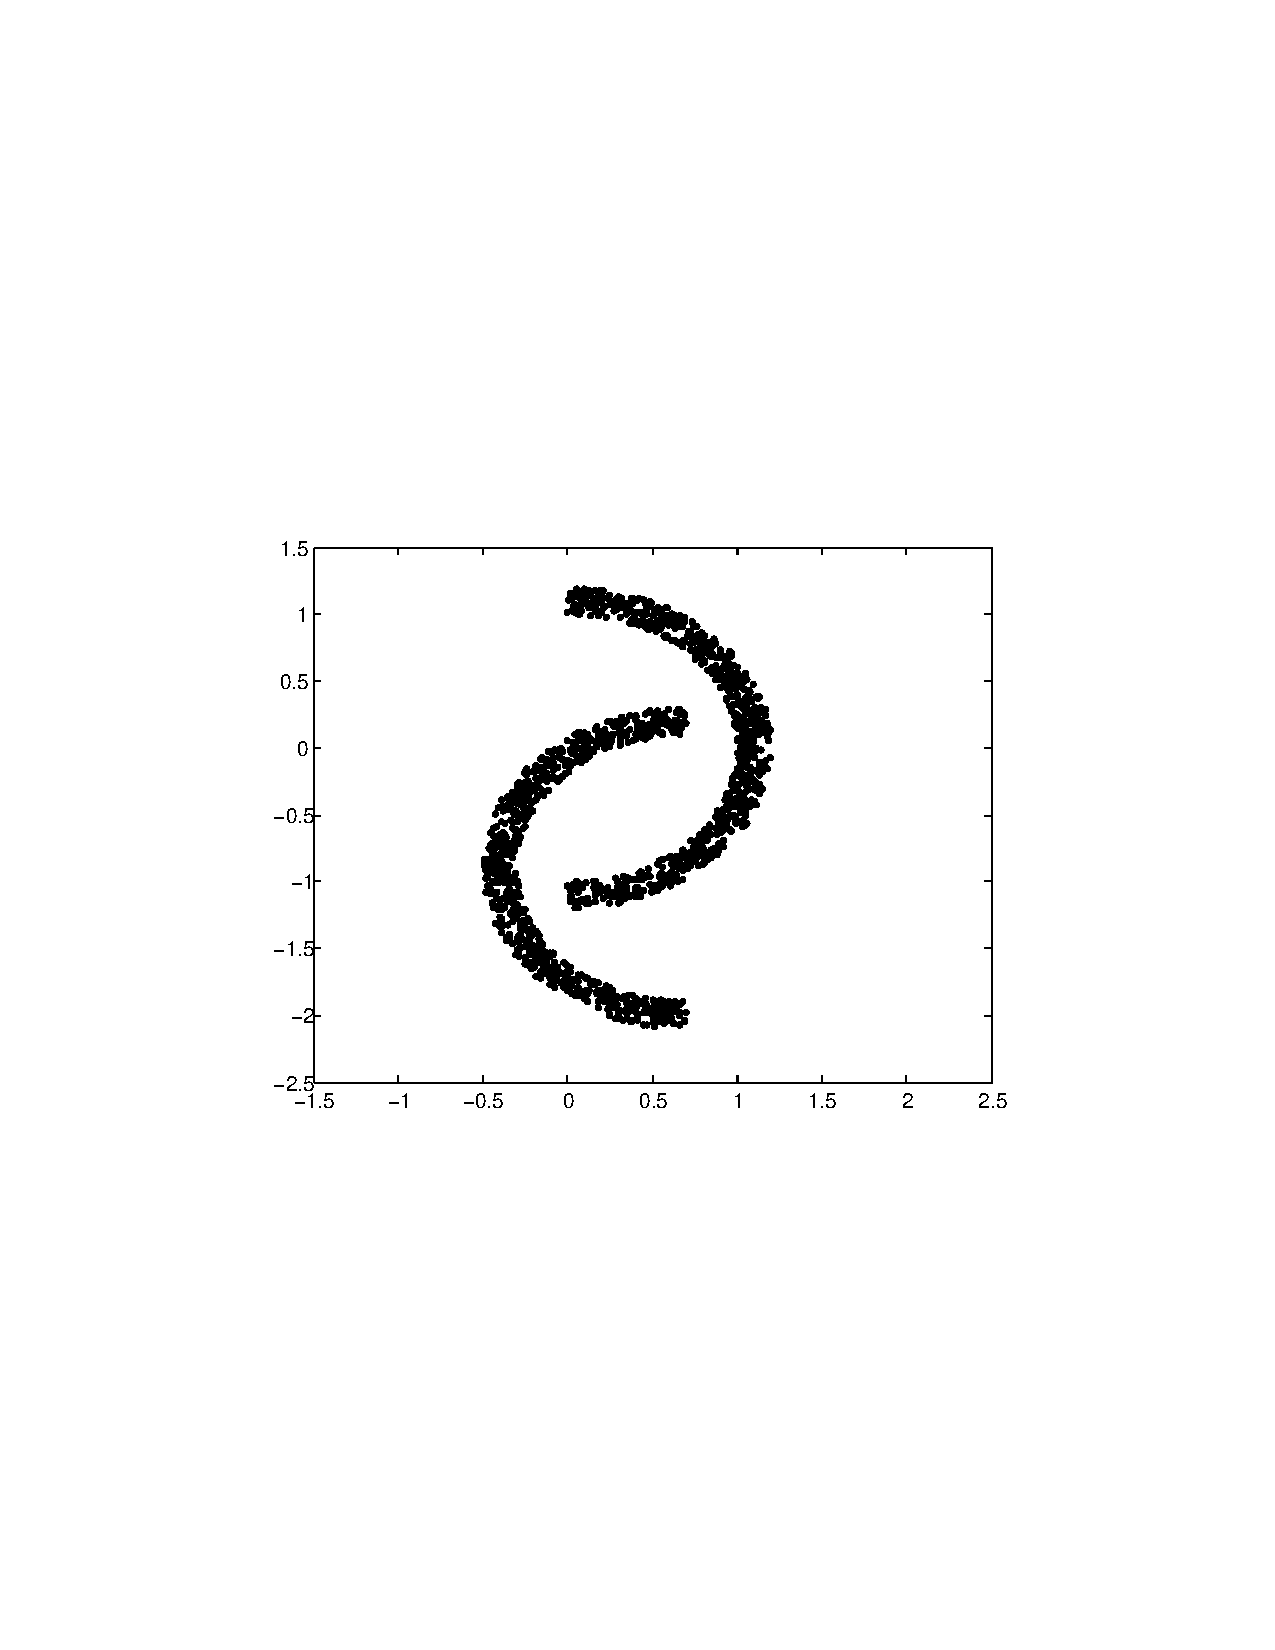
\includegraphics[trim = 0mm 90mm 0mm 90mm, clip, width = \linewidth]{clustering}

\vspace{1cm}



%----------------------------------------------------------------------------------
\section{Programming: Image compression [30 pts]}

In this programming assignment, you are going to apply clustering algorithms for image compression. Before starting this assignment, we strongly recommend reading PRML Section 9.1.1, page 428 -- 430.

To ease your implementation, we provide a skeleton code containing image processing part. \texttt{homework1.m} is designed to read an RGB bitmap image file, then cluster pixels with the given number of clusters $K$. It shows converted image only using $K$ colors, each of them with the representative color of centroid. To see what it looks like, you are encouraged to run \texttt{homework1(`beach.bmp', 3)} or \texttt{homework1(`football.bmp', 2)}, for example.

Your task is implementing the clustering parts with two algorithms: \emph{$K$-means} and \emph{$K$-medoids}. We learned and demonstrated $K$-means in class, so you may start from the sample code we distributed.

The file you need to edit is \texttt{mykmeans.m} and \texttt{mykmedoids.m}, provided with this homework. In the files, you can see it calls Matlab function \texttt{kmeans} initially. Comment this line out, and implement your own in the files. You would expect to see similar result with your implementation of $K$-means, instead of \texttt{kmeans} function in Matlab.

\subsubsection*{$K$-medoids}

In class, we learned that the basic $K$-means works in Euclidean space for computing distance between data points as well as for updating centroids by arithmetic mean. Sometimes, however, the dataset may work better with other distance measures. It is sometimes even impossible to compute arithmetic mean if a feature is categorical, e.g, gender or nationality of a person. With $K$-medoids, you choose a representative data point for each cluster instead of computing their average.

Given $N$ data points $\text x^n (n = 1, ..., N)$, $K$-medoids clustering algorithm groups them into $K$ clusters by minimizing the distortion function $J = \sum_{n=1}^N \sum_{k=1}^K r^{nk} D(\text x^n, \mu^k)$,
where $D(\text x, \text y)$ is a distance measure between two vectors $\text x$ and $\text y$ in same size (in case of $K$-means, $D(x, y) = \| \text x - \text y \|^2$), $\mu^k$ is the center of $k$-th cluster; and $r^{nk} = 1$ if $\text x^n$ belongs to the $k$-th cluster and $r^{nk} = 0$ otherwise. In this exercise, we will use the following iterative procedure:

\begin{itemize}
  \item Initialize the cluster center $\mu^k$, $k = 1, ..., K$.
  \item Iterate until convergence:
  \begin{itemize}
    \item Update the cluster assignments for every data point $\text x^n$: $r^{nk} = 1$ if $k = \argmin_j D(\text x^n, \mu^j)$, and $r^{nk} = 0$ otherwise.
    \item Update the center for each cluster $k$: choosing another representative if necessary.
  \end{itemize}
\end{itemize}

There can be many options to implement the procedure; for example, you can try many distance measures in addition to Euclidean distance, and also you can be creative for deciding a better representative of each cluster. We will not restrict these choices in this assignment. You are encouraged to try many distance measures as well as way of choosing representatives.


\subsubsection*{Formatting instruction}

Both \texttt{mykmeans.m} and \texttt{mykmedoids.m} take input and output format as follows. You should not alter this definition, otherwise your submission will print an error, which leads to zero credit.\\

\textbf{Input}
\begin{itemize}
  \item \texttt{pixels}: the input image representation. Each row contains one data point (pixel). For image dataset, it contains 3 columns, each column corresponding to Red, Green, and Blue component. Each component has an integer value between 0 and 255.
  \item \texttt{K}: the number of desired clusters. Too high value of $K$ may result in empty cluster error. Then, you need to reduce it.
\end{itemize}

\textbf{Output}
\begin{itemize}
  \item \texttt{class}: cluster assignment of each data point in pixels. The assignment should be 1, 2, 3, etc. For $K = 5$, for example, each cell of class should be either 1, 2, 3, 4, or 5. The output should be a column vector with \texttt{size(pixels, 1)} elements.
  \item \texttt{centroid}: location of $K$ centroids (or representatives) in your result. With images, each centroid corresponds to the representative color of each cluster. The output should be a matrix with $K$ rows and 3 columns. The range of values should be [0, 255], possibly floating point numbers.
\end{itemize}

\subsubsection*{Hand-in}
Both of your code and report will be evaluated. Upload \texttt{mykmeans.m} and \texttt{mykmedoids.m} files with your implementation. In your report, answer to the following questions:
\begin{enumerate}
  \item Within the $K$-medoids framework, you have several choices for detailed implementation. Explain how you designed and implemented details of your $K$-medoids algorithm, including (but not limited to) how you chose representatives of each cluster, what distance measures you tried and chose one, or when you stopped iteration.
  \item Attach a picture of your own. We recommend size of $320 \times 240$ or smaller.
  \item Run your $K$-medoids implementation with the picture you chose above, with several different $K$. (e.g, small values like 2 or 3, large values like 16 or 32) What did you observe with different $K$? How long does it take to converge for each $K$?
  \item Run your $K$-medoids implementation with different initial centroids/representatives. Does it affect final result? Do you see same or different result for each trial with different initial assignments? (We usually randomize initial location of centroids in general. To answer this question, an intentional poor assignment may be useful.)
  \item Repeat question 2 and 3 with $K$-means. Do you see significant difference between $K$-medoids and $K$-means, in terms of output quality, robustness, or running time?
\end{enumerate}


\subsubsection*{Note}
\begin{itemize}
  \item You may see some error message about empty clusters even with Matlab implementation, when you use too large $K$. Your implementation should treat this exception as well. That is, do not terminate even if you have an empty cluster, but use smaller number of clusters in that case.

  \item We will grade using test pictures which are not provided. We recommend you to test your code with several different pictures so that you can detect some problems that might happen occasionally. 

  \item If we detect copy from any other student's code or from the web, you will not be eligible for any credit for the entire homework, not just for the programming part. Also, directly calling Matlab function \texttt{kmeans} or other clustering functions is not allowed.
\end{itemize}

%\bibliographystyle{plain}
%\bibliography{temp,externalPapers,groupPapers}

\end{document}
